\section{Analysis}
\label{sec:Auswertung}
To compute the isobaric heat capacity $C_p$, the molar mass of copper $M = 63.546\frac{\text{g}}{\text{mol}}$, the sample's mass $m = \text{g}$, the energy $E$ that was added to the system and the temperature difference $\Delta T$ that was achieved by adding this amount of energy are required. \\
To get the energy, the voltage $U$, the current $I$ and the time interval $\Delta t$ over which energy was added to the system were measured. To get the temperature $T$ of the system, the thermometre's resistance $R$ was measured, since the temperature can then be measured via
\begin{aquation}
  T\lbr R \rbr = 0.00134 R^2 + 2.296 R - 243.02 \tp
\end{aquation}
The resistance steps have been chosen carefully to ensure that $\Delta T$ is always $10\text{K}$. To get the isobaric heat capacity, the measured and computed values have to be plugged into the equation 
\begin{aquation}
  C_p &= \frac{M}{m} \frac{E}{\Delta T}\tp
\end{aquation}
The isochoric heat capacity is related to the isobaric heat capacity via 
\begin{aquation}
  C_V &= C_p - 9 V_0 \alpha^2 \kappa T \tc
\end{aquation}
as has been noted in \autoref{eq:cp-cv}.\\
The resulting heat capacities can be found in \autoref{fig:molar_heat}.\\
\begin{figure}
  \centering
  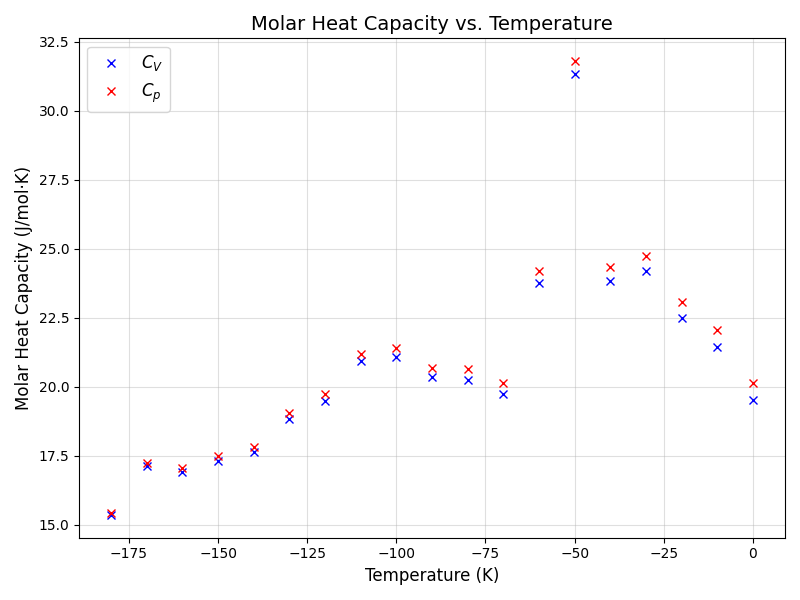
\includegraphics[width=0.8\textwidth]{figures/CVvsCP.png}
  \caption{Comparison between $C_v$ and $C_p$}
  \label{fig:molar_heat}
\end{figure}
Here, $\kappa = 137.8 \text{GPa}$ is the bulk module, $V_0 = 7.092 \times 10^6 \frac{\text{m}^3}{\text{mol}}$ the molar volume and $\alpha$ the volumetric expansion. The latter one's values given in \cite{Anleitung47} do not match the temperatures that have been measured in this experiment. For this reason, a linear interpolation has to be performed, yielding approximate values for $\alpha$ at the measured temperature. These approximates are listed in \autoref{tab:alpha}\\
The results for the heat capacities can be found in \autoref{tab:Cp+CV}.
\begin{table}
  \centering
  \begin{tabular}{rrrr}
\toprule
$T$ / °C & $E$ / J & $C_p$ / $\frac{\text{J}}{\text{mol}\cdot\text{K}}$ & $C_V$ / $\frac{\text{J}}{\text{mol}\cdot\text{K}}$ \\
\midrule
-180.00 & 830.96 & 15.44 & 15.36 \\
-170.00 & 927.58 & 17.24 & 17.13 \\
-160.00 & 917.38 & 17.05 & 16.91 \\
-150.00 & 940.83 & 17.48 & 17.32 \\
-140.00 & 959.08 & 17.82 & 17.63 \\
-130.00 & 1026.15 & 19.07 & 18.84 \\
-120.00 & 1062.44 & 19.74 & 19.49 \\
-110.00 & 1141.43 & 21.21 & 20.93 \\
-100.00 & 1152.03 & 21.41 & 21.09 \\
-90.00 & 1113.17 & 20.68 & 20.34 \\
-80.00 & 1110.73 & 20.64 & 20.27 \\
-70.00 & 1084.14 & 20.14 & 19.74 \\
-60.00 & 1301.73 & 24.19 & 23.75 \\
-50.00 & 1711.84 & 31.81 & 31.34 \\
-40.00 & 1309.45 & 24.33 & 23.83 \\
-30.00 & 1331.94 & 24.75 & 24.21 \\
-20.00 & 1241.91 & 23.08 & 22.51 \\
-10.00 & 1186.71 & 22.05 & 21.45 \\
-0.00 & 1084.19 & 20.15 & 19.51 \\
\bottomrule
\end{tabular}

  \caption{Values for the isobaric heat capacity $C_p$ and the isochorich heat capacity $C_V$.}
  \label{tab:Cp+CV}
\end{table}
\begin{table}
  \centering
  \begin{tabular}{rr}
\toprule
$T$ / °C & $\alpha$ / $10^{-6} \frac{1}{\text{K}}$ \\
\midrule
-180.00 & 10.04 \\
-170.00 & 10.96 \\
-160.00 & 11.70 \\
-150.00 & 12.29 \\
-140.00 & 12.81 \\
-130.00 & 13.29 \\
-120.00 & 13.69 \\
-110.00 & 14.01 \\
-100.00 & 14.33 \\
-90.00 & 14.58 \\
-80.00 & 14.81 \\
-70.00 & 15.03 \\
-60.00 & 15.26 \\
-50.00 & 15.46 \\
-40.00 & 15.64 \\
-30.00 & 15.80 \\
-20.00 & 15.96 \\
-10.00 & 16.15 \\
-0.00 & 16.28 \\
\bottomrule
\end{tabular}

  \caption{Values for the volumetric expansion $\alpha$ received via linear extrapolation.}
  \label{tab:alpha}
\end{table}

\subsection{The Debye Temperature}
The Debye temperature can be computed via the table in \autoref{fig:debye}. The first column is the significand and the first line is the mantisse of $\frac{\Theta_D}{T}$. The remaining values are the corresponding heat capacities $C_V$. Thus, to find a $\frac{\Theta_D}{T}$-value for a $C_V$, the closest $C_V$ has to be found within the table, which makes it possible to read the value from the table.\\
The Debye temperature can then be derived by simply multiplying the value from the table with the according $T$. Doing so results in the values depicted in \autoref{tab:debye_results}. Only values $T<170\text{K}$ have been considered.\\
The mean value for the Debye-temperature is then $\Theta_D = (330.42 \pm 7.11) \text{K}$.
\begin{figure}[h!]
  \centering
  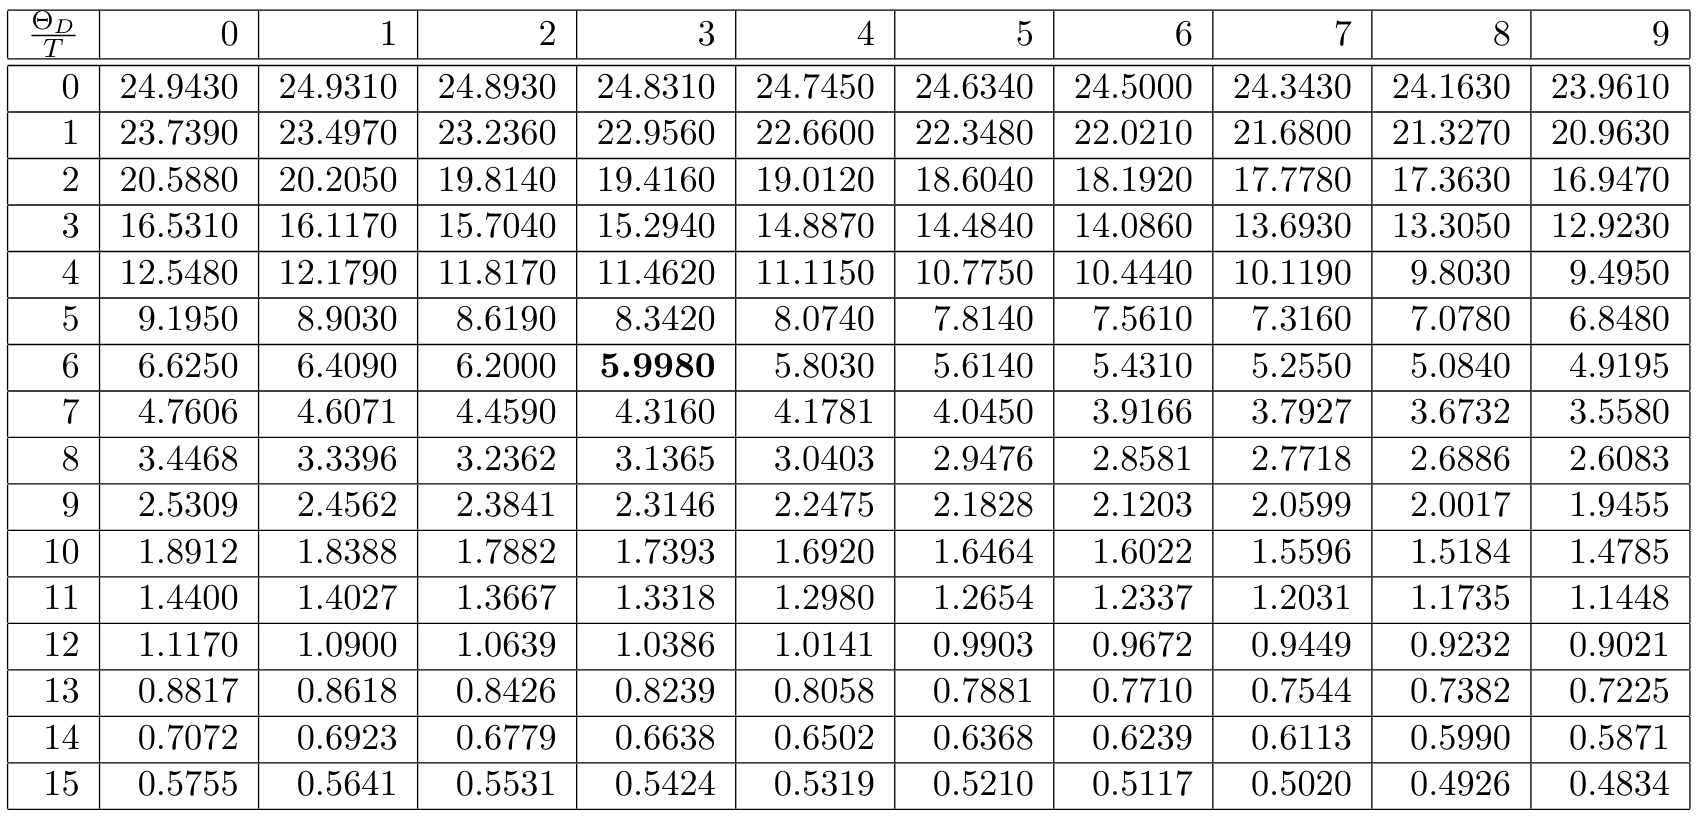
\includegraphics[width=\textwidth]{figures/Debye_values.png}
  \caption{The value of $\frac{\Theta_D}{T}$ can be read off this table. To do so, the closest value for $C_V$ has to be found within the table. Then, $\frac{\Theta_D}{T} = \textit{row}.\textit{column}$}
  \label{fig:debye}
\end{figure}

\begin{table}
  \centering
  \begin{tabular}{rrr}
\toprule
$T$ / °C & $\theta_D/T$ & $\theta_D$ / °C \\
\midrule
-180.00 & 3.30 & 307.39 \\
-170.00 & 2.90 & 299.13 \\
-160.00 & 2.90 & 328.13 \\
-150.00 & 2.80 & 344.82 \\
-140.00 & 2.70 & 359.50 \\
-130.00 & 2.40 & 343.56 \\
-120.00 & 2.30 & 352.24 \\
-110.00 & 1.90 & 309.98 \\
-100.00 & 1.90 & 328.98 \\
\bottomrule
\end{tabular}

  \caption{Resulting Debye temperature $\Theta_D$}
  \label{tab:debye_results}
\end{table}

\subsection{The Debye Frequency}
The Debye frequency is 
\begin{aquation}
  \omega_D &= \frac{v_m k_D}{2\pi} \tp
\end{aquation}
Plugging in the Debye wavenumber 
\begin{aquation}
  k_\text{D} &= \lbr 6\pi^2 \frac{N_A}{V_0}\rbr^{1/3}
\end{aquation}
and the average speed of sound 
\begin{aquation}
  v_\text{m} &= \lbr \frac{1}{3} \lbs 2 \frac{1}{v_t^3} + \frac{1}{v_l^3} \rbs \rbr^{-1/3}
\end{aquation}
into this, the full expression becomes 
\begin{aquation}
  \omega_\text{D} &= \frac{1}{2\pi} \lbr 18\pi^2 \frac{N_A}{V_0} \lbs 2 \frac{1}{v_t^3} + \frac{1}{v_l^3} \rbs^{-1} \rbr^{1/3} \tp
\end{aquation}
Here, $N_A$ is the Avogadro-constant, and the velocities are $v_t = 4.7 \text{km/h}$ and $v_l = 2.26 \text{km/h}$. Plugging all these values in, the final result becomes $\omega_D = 43.39\cdot 10^{12} \frac{1}{1}{s}$, and thus, via 
\begin{aquation}
  \Theta_D &= \frac{\hbar \omega_D}{k_B}
\end{aquation}
the resulting Debye temperature is $\Theta_D = 330.7\text{K}$. 